%%%%%%%%%%%%%%%%%%%%%%%%%%%%%%%%%%%%%%%%%
% University/School Laboratory Report
% LaTeX Template
% Version 3.1 (25/3/14)
%
% This template has been downloaded from:
% http://www.LaTeXTemplates.com
%
% Original author:
% Linux and Unix Users Group at Virginia Tech Wiki 
% (https://vtluug.org/wiki/Example_LaTeX_chem_lab_report)
%
% License:
% CC BY-NC-SA 3.0 (http://creativecommons.org/licenses/by-nc-sa/3.0/)
%
%%%%%%%%%%%%%%%%%%%%%%%%%%%%%%%%%%%%%%%%%

%----------------------------------------------------------------------------------------
%	PACKAGES AND DOCUMENT CONFIGURATIONS
%----------------------------------------------------------------------------------------

\documentclass{article}

\usepackage[version=3]{mhchem} % Package for chemical equation typesetting
\usepackage{siunitx} % Provides the \SI{}{} and \si{} command for typesetting SI units
\usepackage{graphicx} % Required for the inclusion of images
\usepackage{natbib} % Required to change bibliography style to APA
\usepackage{amsmath} % Required for some math elements 
\usepackage{enumerate} % Required for the enumerate function
\usepackage[siunitx]{circuitikz} % Required for the drawing of circuit diagrams
\usepackage{caption}
\usepackage{graphicx}
\usepackage{subcaption}
\usepackage{xfrac}
\usepackage{float}
\usepackage{enumitem}
\usepackage{chemgreek}
\usepackage{pgfplots}

\setlength\parindent{0pt} % Removes all indentation from paragraphs

\renewcommand{\labelenumi}{\alph{enumi}.} % Make numbering in the enumerate environment by letter rather than number (e.g. section 6)

%\usepackage{times} % Uncomment to use the Times New Roman font

\graphicspath{{./fig/}}

%----------------------------------------------------------------------------------------
%	DOCUMENT INFORMATION
%----------------------------------------------------------------------------------------

\title{Power Systems Analysis \\ Practical 2 \\ ENG474} % Title

\author{Shane \textsc{Reynolds}} % Author name

\date{\today} % Date for the report

\begin{document}

\maketitle % Insert the title, author and date

\begin{center}
\begin{tabular}{l r}
Date Performed: & June 22, 2017 \\ % Date the experiment was performed
Instructor: & Dr Kamal Debnath % Instructor/supervisor
\end{tabular}
\end{center}

% If you wish to include an abstract, uncomment the lines below
% \begin{abstract}
% Abstract text
% \end{abstract}

%----------------------------------------------------------------------------------------
%	SECTION 1
%----------------------------------------------------------------------------------------
\section{Objective}
The principal object of this practical is two fold: firstly, the real and reactive power is observed in a three-phase transmission line with known passive loads. Secondly, the voltage regulation at the receiver end is observed as a function of the type of load.


%----------------------------------------------------------------------------------------
%	SECTION 2
%----------------------------------------------------------------------------------------
\section{Theory}
The model of a transmission line can be thought of in the context of the three main passive elements: resistance, inductance, and capacitance. The resistance in the conductors prevents the flow of current, and results in power loss in the form of dissipated heat. Since there is a current flowing in a current carrying conductor, this creates a magnetic field, which results in an inductance being present in the line. Finally, the voltage potential difference increase between the line and the ground, which is seen when the line is being used for power transmission can be modelled by a capacitor.
\begin{figure}[H]
	\centering
	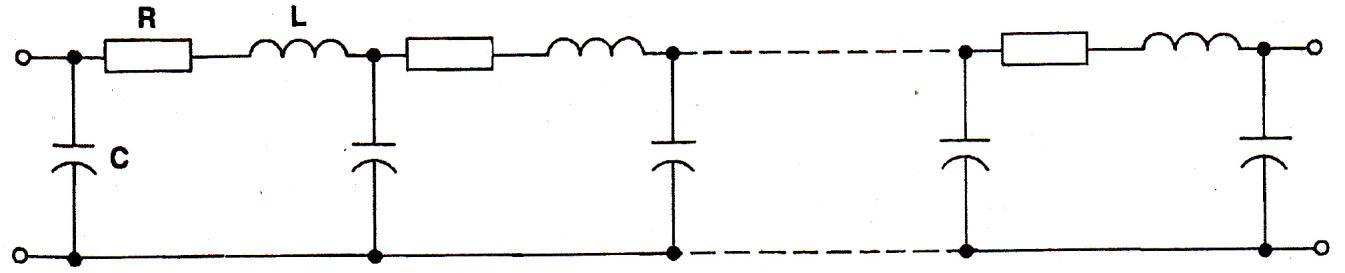
\includegraphics[scale=0.7]{fig1}
	\caption{Model of a transmission line}
\end{figure}

Assuming a uniform distribution of the resistance, inductance and capacitance, the transmission line model can be thought of as simple passive devices distributed uniformly along the length of the transmission line, as shown in Figure 1. When modelling low frequency transmission lines, we simplify this model further by using a single resistor, a single inductor, and two capacitors of equal value. This model is shown in Figure 2.
\begin{figure}[H]
	\centering
	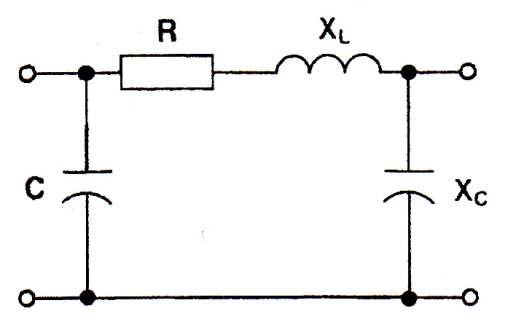
\includegraphics[scale=0.8]{fig2}
	\caption{Model of a transmission line for low frequency networks}
\end{figure}

We note that when using the model seen in Figure 2, the resistance, $R$, is found by summing all of the individual resistances in the conductor. Similarly, we can perform the same operation to find the inductance, $L$. The capacitances seen in Figure 1, are in parallel, however, in this configuration we sum all the individual capacitances and divide by two to arrive at values for the capacitance, $C$, used in the model shown in Figure 2.

%----------------------------------------------------------------------------------------
%	SECTION 3
%----------------------------------------------------------------------------------------
\section{Process \& Results}

Two Wattmeters were connected in series to the variable Three Phase 415$\si{\volt}$ section of a power supply. A star connected 1200 $\si{\ohm}$ inductive load was connected at the end of the transmission line, as shown in Figure 3. The power supply was adjusted to 415 $\si{\volt}$.
\begin{figure}[H]
	\centering
	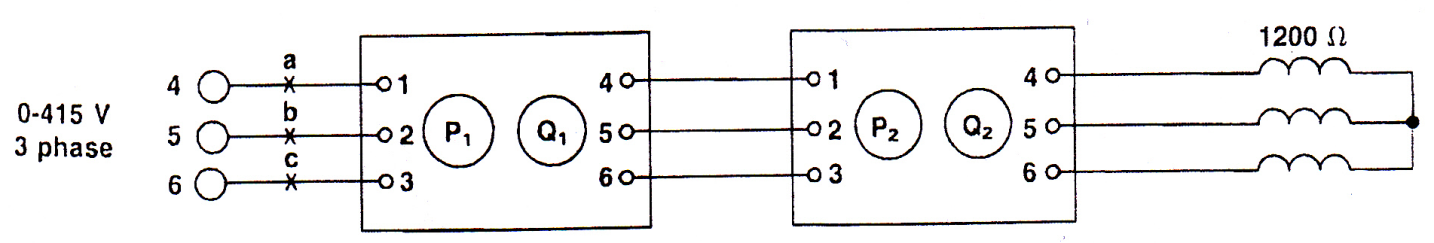
\includegraphics[scale=0.7]{fig3}
	\caption{Diagram of the practical set up}
\end{figure}

The readings from the meters are as follows:
\begin{center}
	\fbox{$P_1 = 20 \si{\watt}, \quad Q_1 = 140 \si{VAR}, \quad$
	$P_2 = 10 \si{\watt}, \quad Q_2 = 100 \si{VAR}$}
\end{center}

The transmission circuit was then set up using the model shown in Figure 4. Notably, voltmeters which are measuring the line to line voltages have been implemented before the first Wattmeter and after the second Wattmeter, before the inductive load. In this instance, the transmission line impedance was set to 400$\si{\ohm}$.

%----------------------------------------------------------------------------------------
%	SECTION 4
%----------------------------------------------------------------------------------------
\section{Discussion}




%----------------------------------------------------------------------------------------
%	SECTION 5
%----------------------------------------------------------------------------------------
\section{Conclusion}




\end{document}